\documentclass{beamer}
\usepackage[utf8]{inputenc}
\usepackage[utf8]{inputenc}
\usepackage{mathtools}
\usepackage{amsmath,amsfonts,amssymb,amsthm,bm}
\usepackage{nccmath}
\usepackage{multimedia}
\usepackage{hyperref}
\usepackage{svg}
\usepackage{graphicx}
\usepackage{media9}

\usetheme{CambridgeUS}
\usecolortheme{default}

%\setbeamertemplate{sections/subsections in toc}[sections numbered]
\useinnertheme{rectangles} % adds squared bullets to TOC

\setbeamertemplate{itemize item}[triangle]
\setbeamertemplate{enumerate item}[circle]
%\setbeamercolor*{enumerate item}{fg=red}
%\setbeamercolor*{enumerate subitem}{fg=red}
%\setbeamercolor*{enumerate subsubitem}{fg=red}
%\setbeamercolor*{itemize item}{fg=red}
%\setbeamercolor*{itemize subitem}{fg=red}
%\setbeamercolor*{itemize subsubitem}{fg=red}

%------------------------------------------------------------
%This block of code defines the information to appear in the
%Title page
\title[Double pendulum] {The double pendulum}
\subtitle{Is it really that chaotic ?}

\author[Vincent Degrooff] % (optional)
{Vincent Degrooff}

\institute[EPL] % (optional)
{
  LINMA2361 - Nonlinear dynamical systems\\
  EPL UCLouvain
}

\date[20 January 2022] % (optional)
{Project presentation, January 2022}

%\logo{\includesvg[height=4mm]{../figures/Logo_EPL.svg}}

%End of title page configuration block
%------------------------------------------------------------



%------------------------------------------------------------
%The next block of commands puts the table of contents at the 
%beginning of each section and highlights the current section:

\AtBeginSection[]
{
  \begin{frame}
    \frametitle{Table of Contents}
    \tableofcontents[currentsection]
  \end{frame}
}
%------------------------------------------------------------


\begin{document}

%The next statement creates the title page.
\frame{\titlepage}

\begin{frame}{Introduction: A chaotic trajectory}
    \centering
    \movie[externalviewer]{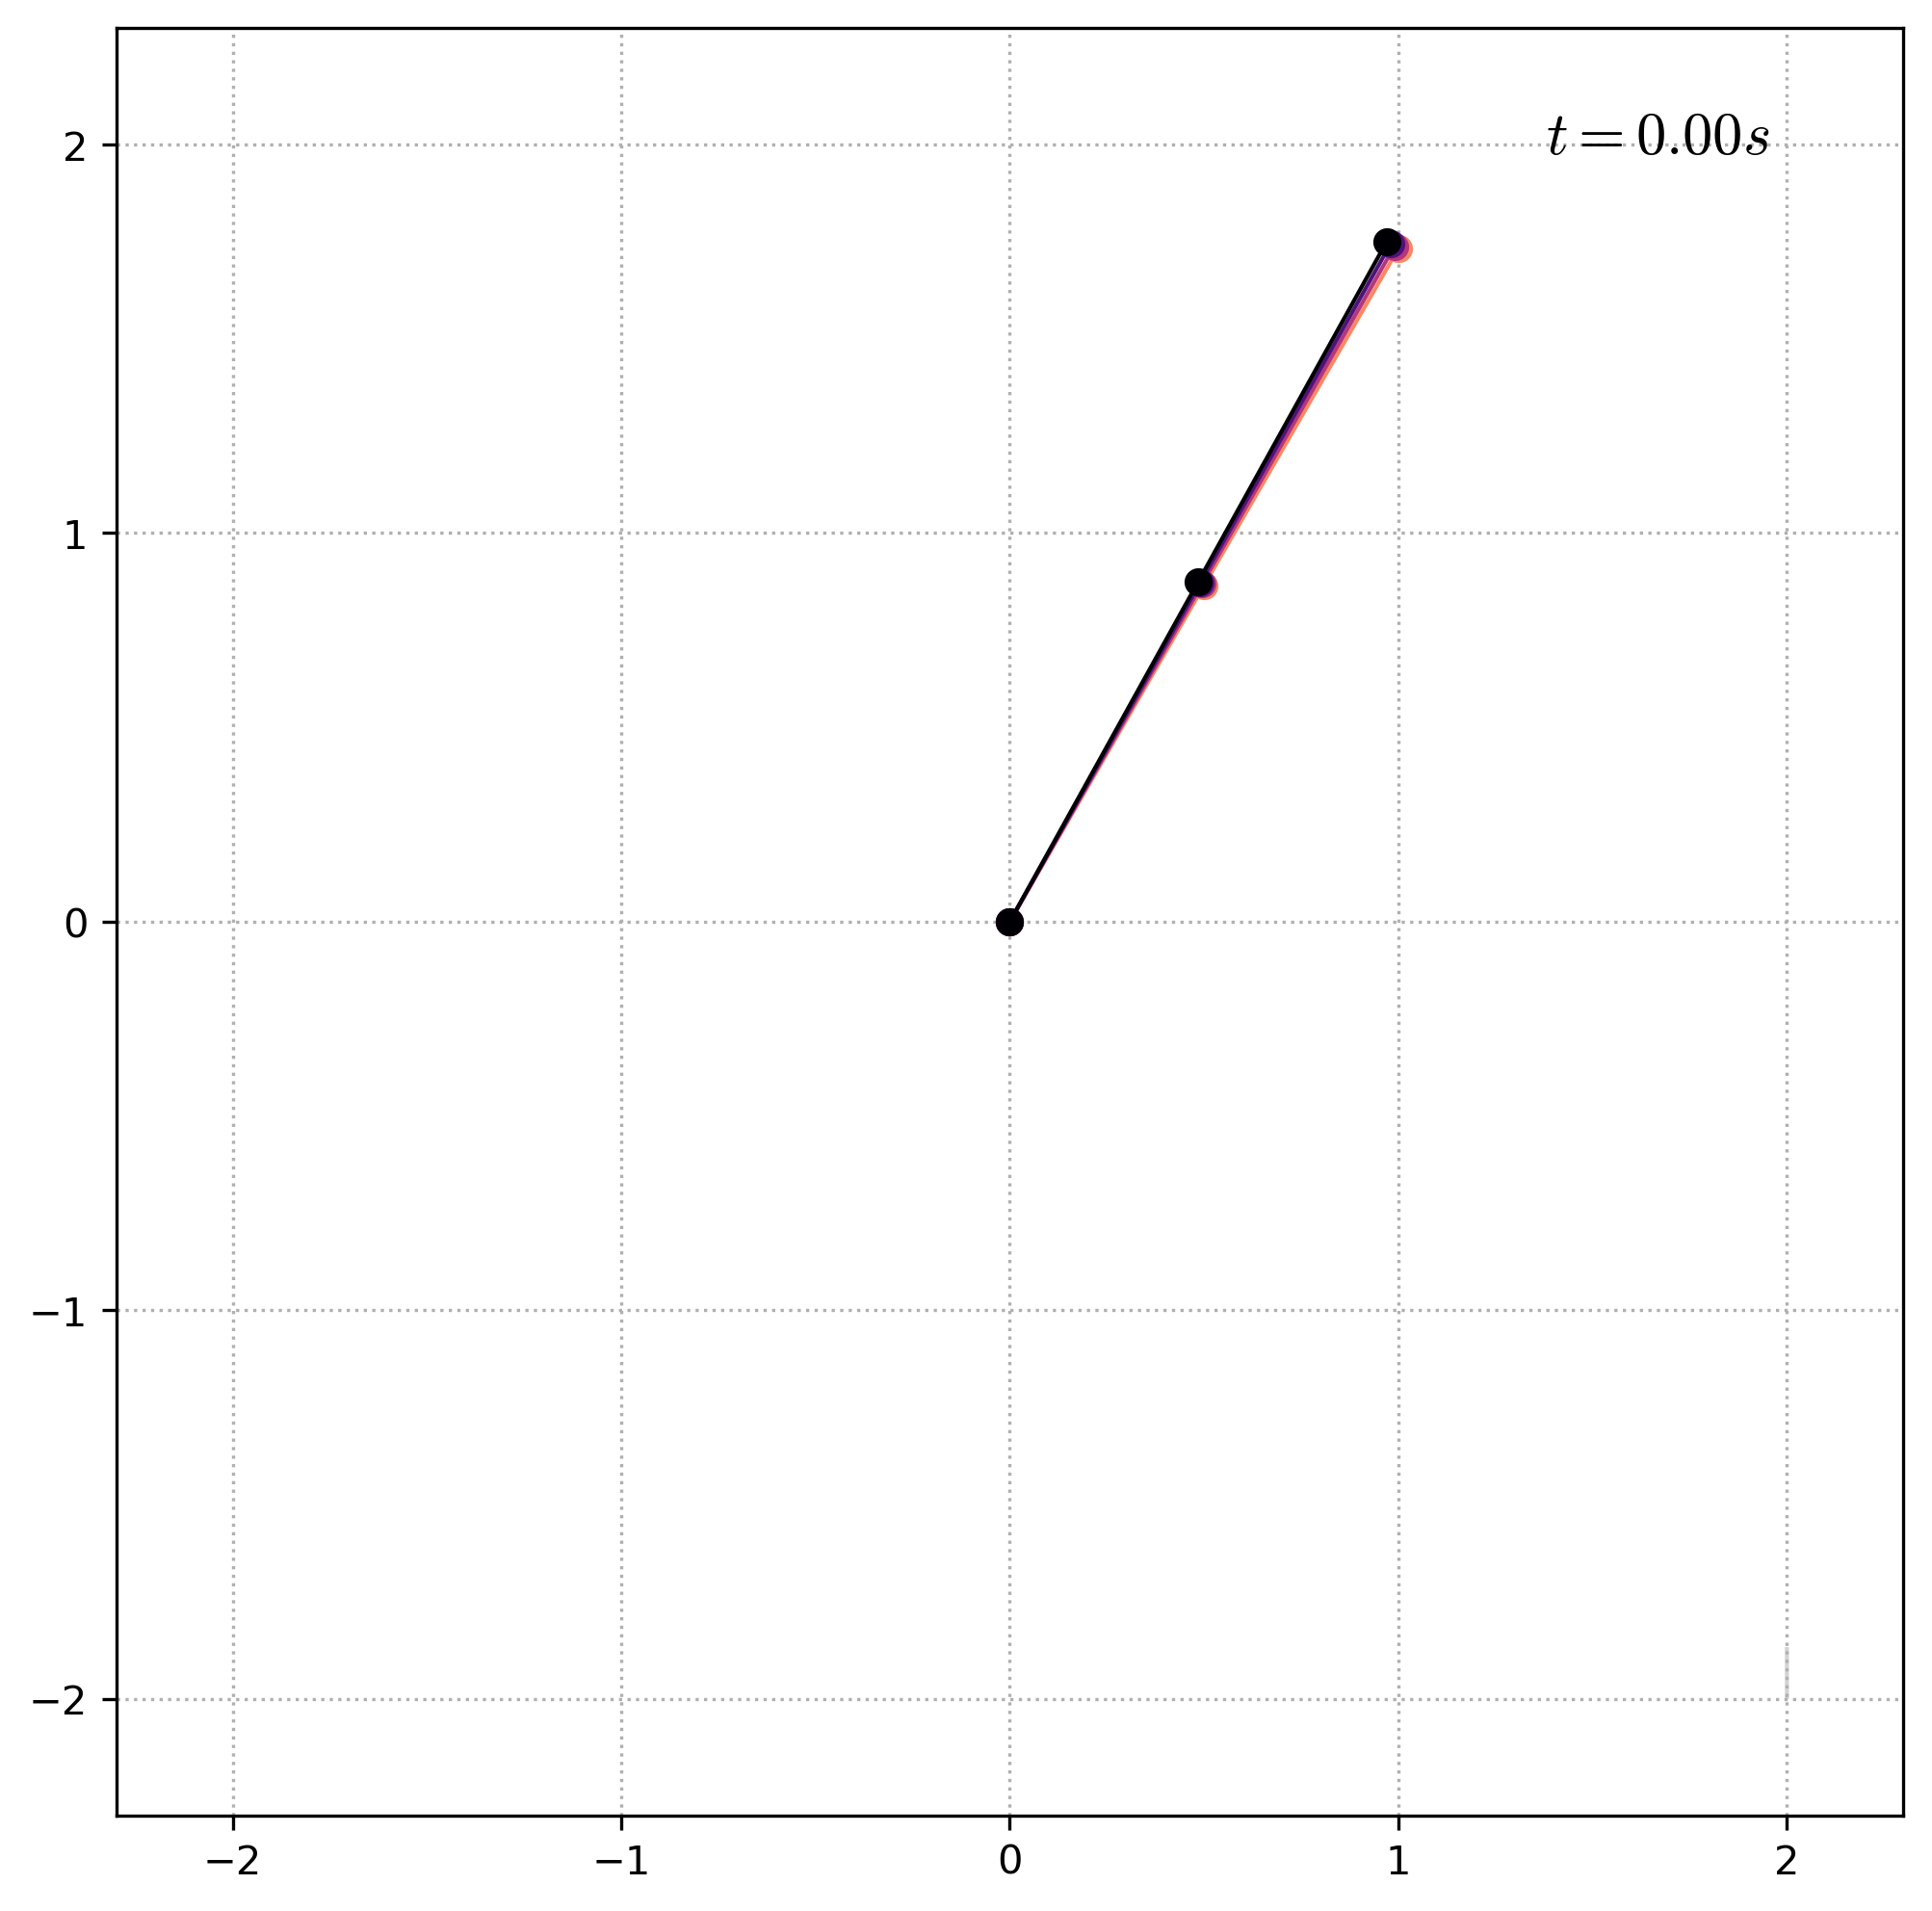
\includegraphics[height=7cm, keepaspectratio]{../animations/fig_chaos.png}}{../animations/multiple_pendulum_chaos.mp4}
\end{frame}

\begin{frame}{Introduction: A non-chaotic trajectory}
    \centering
    \movie[externalviewer]{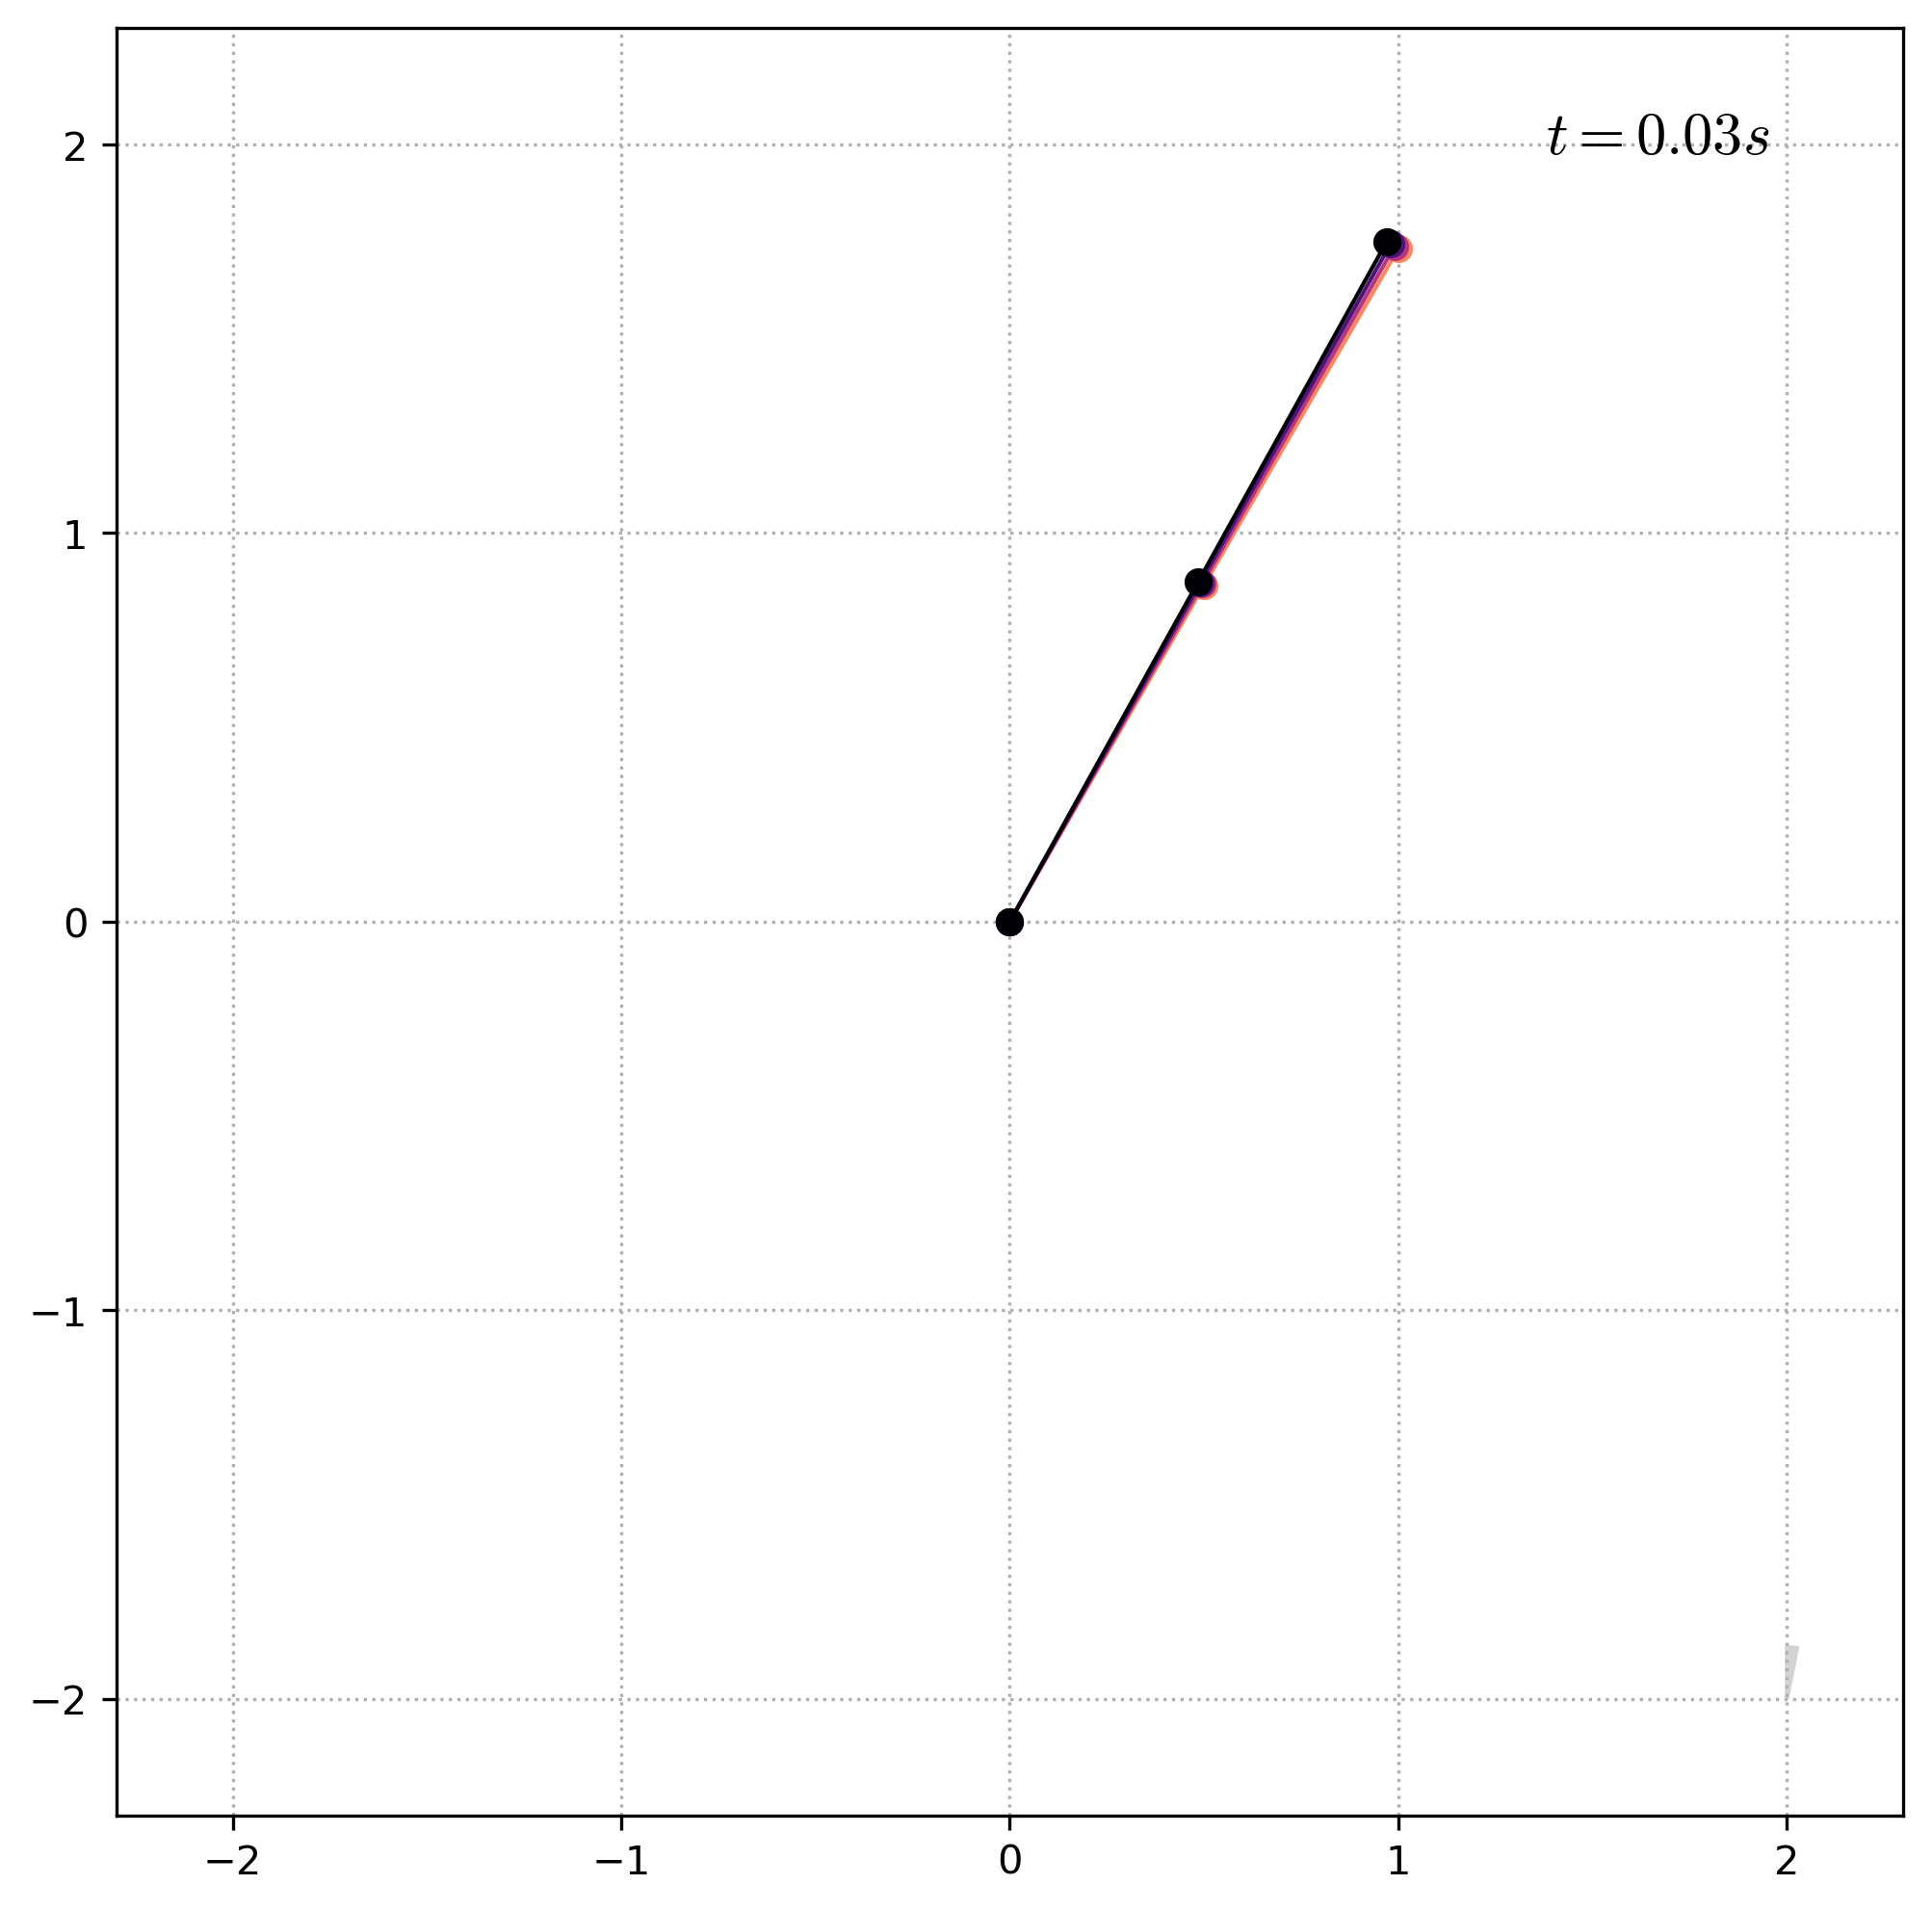
\includegraphics[height=7cm, keepaspectratio]{../animations/fig_quasi.png}}{../animations/multiple_pendulum_quasi.mp4}
\end{frame}

%---------------------------------------------------------

\begin{frame}
\frametitle{Table of Contents}
\tableofcontents
\end{frame}

%---------------------------------------------------------

\section{Modeling of the mechanical system}

\begin{frame}{Description}

\begin{figure}
    \centering
    \includesvg[height=6.5cm]{../figures/description.svg}
    %\caption{Description of the double pendulum.}
    %\label{fig:description}
\end{figure}
\end{frame}

\begin{frame}{Equations of motion}
The Lagrangian of the system:
\begin{small}
\begin{align*}
    \mathcal{L}&=\mathcal{K}-\mathcal{U}\\
    \mathcal{K} &= \frac{m_1}{2} \ell_1^2 \dot \varphi_1^2 + \frac{m_2}{2} \left[ \ell_1^2\, \dot \varphi_1^2 + \ell_2^2\, \dot \varphi_2^2  + 2 \ell_1 \ell_2 \, \dot \varphi_1 \dot \varphi_2 \cos{\overbrace{\left(\varphi_1 - \varphi_2\right)}^{\coloneqq \theta}}\right] \\
    \mathcal{U} &= \left[\left(m_1+m_2\right)g \ell_1 \left(1 - \cos{\varphi_1}\right) + m_2 g \ell_2 \left(1 - \cos \varphi_2\right)\right]
\end{align*}
\end{small}
\pause

The Euler-Lagrange equations:
\begin{align*}
    \frac{\mathrm{d}}{\mathrm{d}t} \left(\frac{\partial \mathcal{L}}{\partial \dot \varphi_i}\right) = \frac{\partial \mathcal{L}}{\partial \varphi_i}
\end{align*}
\pause

\begin{small}
\begin{align*}
    (m_1+m_2) \ell_1 \ddot \varphi_1 + m_2 \ell_2 \ddot \varphi_2 \cos \theta &= -m_2 \ell_2 \dot \varphi_2^2 \sin \theta - (m_1+m_2) g \sin \varphi_1\\
    \ell_1 \ddot \varphi_1 \cos \theta + \ell_2 \ddot \varphi_2 &= \ell_1 \dot \varphi_1^2\sin{\theta} - g \sin \varphi_2
\end{align*}
\end{small}

%\begin{itemize}
%    \item<1-> Text visible on slide 1
%    \item<2-> Text visible on slide 2
%    \item<3> Text visible on slides 3
%    \item<4-> Text visible on slide 4
%\end{itemize}

\end{frame}

\begin{frame}{State-space formulation}
A choice of nondimensionalization ?
\pause
\begin{align*}
    \lambda = \frac{\ell_2}{\ell_1} \qquad \mu  = \frac{m_2}{m_1+m_2} \qquad \tau = \sqrt{\frac{g}{\ell_1}} t\\
\end{align*} \pause

We obtain the following system
\begin{small}
\begin{align*}
    f(x)=
    \frac{\mathrm{d}}{\mathrm{d}t}
    \begin{bmatrix}
        \varphi_1\\[2pt]
        \varphi_2\\[2pt]
        \omega_1\\[2pt]
        \omega_2
    \end{bmatrix} = 
    \begin{bmatrix}
        \omega_1\\[2pt]
        \omega_2\\[2pt]
        \left[\mu \cos \theta (\sin \varphi_2 - \omega_1^2 \sin \theta) - \lambda \mu \omega_2^2 \sin \theta - \sin \varphi_1\right]\frac{1}{1 - \mu \cos^2\theta}\\[2pt]
        \frac{1}{\lambda} \sin \theta \left[\cos \varphi_1 + \omega_1^2 + \lambda \mu \omega_2^2 \cos \theta \right]\frac{1}{1 - \mu \cos^2\theta}\\[2pt]
    \end{bmatrix}
\end{align*}
\end{small}

\end{frame}

%---------------------------------------------------------

\section{Analysis of the equilibria}

\begin{frame}{What about the equilibria}
\begin{itemize}
    \setlength\itemsep{\fill}
    \item How many ?
    \item What coordinates ?
    \item Which one(s) is/are stable ?
\end{itemize}    
\end{frame}

\begin{frame}{Eigenvalues of the 4 equilibria}
\begin{figure}
    \centering
    \includesvg[height=6.5cm]{../figures/eigenvalues/eigenvalues_latex_2.00.svg}
    \begin{small}
    \caption{Eigenvalues for $\lambda=2$ and $\mu\in [0.05, 0.95]$.}
    \end{small}
\end{figure}
\end{frame}

%---------------------------------------------------------

\section{Quasiperiodicity}

\begin{frame}{Simple system}

\begin{example}
\begin{align*}
    \dot \theta_1 = \omega_1\\
    \dot \theta_2 = \omega_2
\end{align*}
\end{example}

\vspace{7mm}
Two possibilities
\begin{itemize}
    \item $\omega_1/\omega_2=p/q$ rational
    \item $\omega_1/\omega_2$ irrational
\end{itemize}
\end{frame}

\begin{frame}{Commensurable frequencies}
    \centering
    \movie[externalviewer]{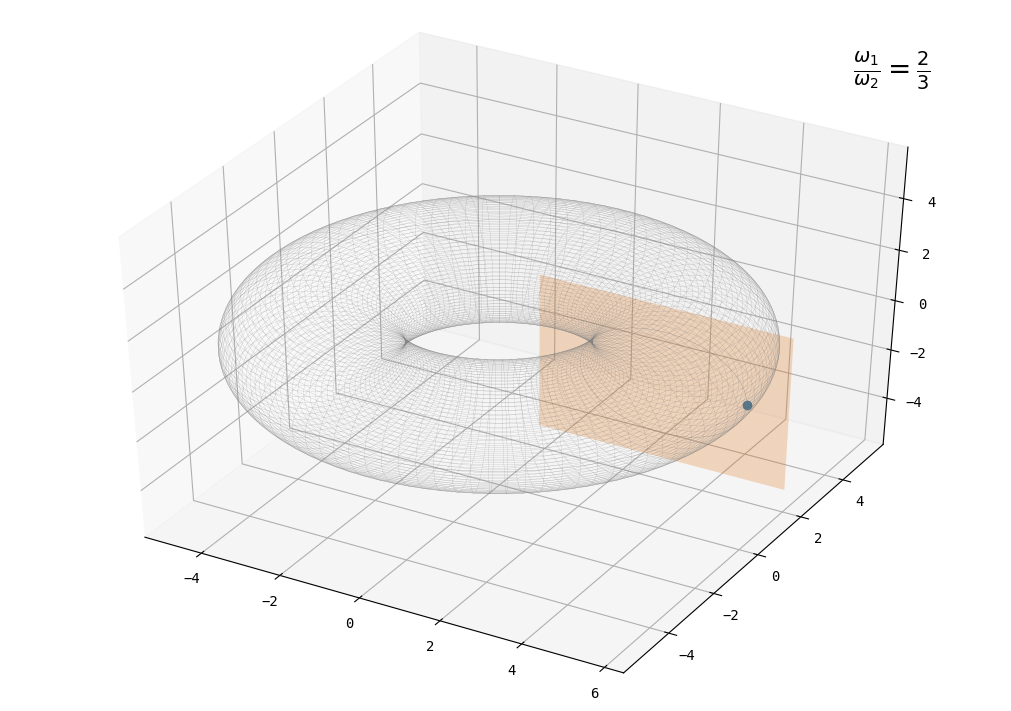
\includegraphics[height=7cm, keepaspectratio]{../animations/fig_torus_periodic.png}}{../animations/poincare_periodic.mp4}
\end{frame}

\begin{frame}{Incommensurable frequencies}
    \centering
    \movie[externalviewer]{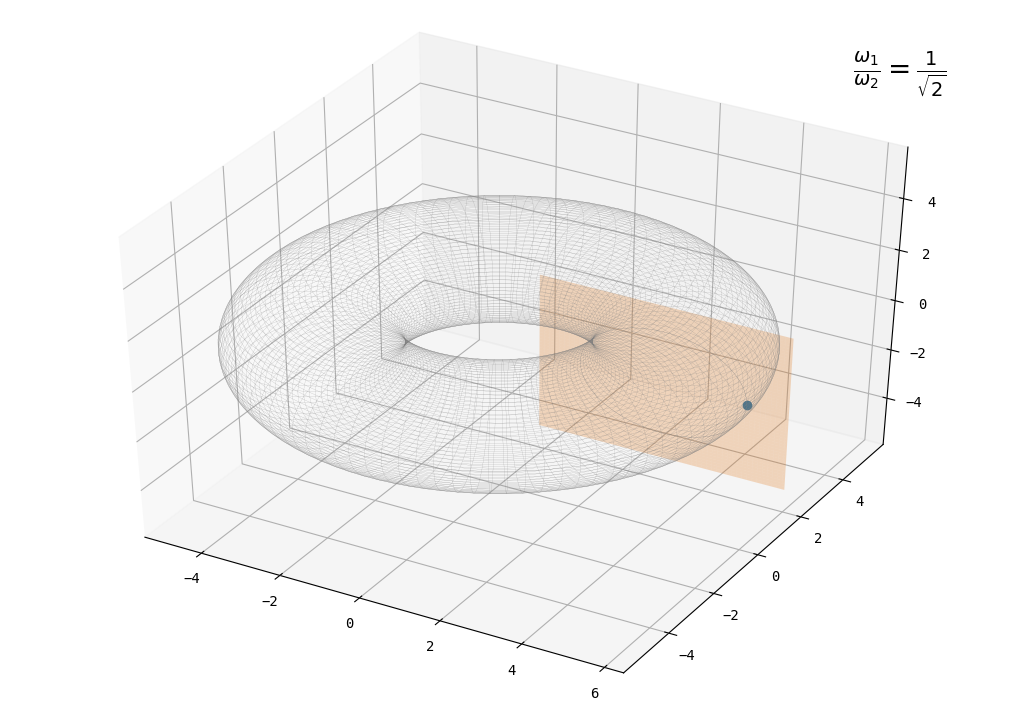
\includegraphics[height=7cm, keepaspectratio]{../animations/fig_torus_quasi.png}}{../animations/poincare_quasi_fast.mp4}
\end{frame}

\begin{frame}{Recap}
\begin{itemize}
    \setlength\itemsep{\fill}
    \item Periodic orbits: finite number of points
    \item Quasiperiodic orbits: curve-filling points
    \item Chaotic orbits: area-filling points
\end{itemize}  
\end{frame}

%---------------------------------------------------------

\section{Poincaré sections}


%---------------------------------------------------------

\begin{frame}{What is a Poincaré section}
    \begin{itemize}
        \item Cannot visualize 4-dimensional state-space
        \item Pick a lower-dimensional slice of the state-space and look for intersection points with the trajectory
    \end{itemize}
    \pause
    
    \vspace{10mm}
    In the case of the double pendulum, section can be defined:
    \begin{align*}
        \varphi_1 &= 0 \qquad \text{and} \qquad \dot \varphi_1 + \mu \lambda \dot \varphi_2 \cos{\varphi_2} > 0\\
        \text{or}\qquad \varphi_2 &= 0 \qquad \text{and} \qquad \dot \varphi_2 + \frac{1}{\lambda} \dot \varphi_1 \cos{\varphi_1} > 0
    \end{align*}
\end{frame}

\begin{frame}{Numerical experiment - low energy}
\begin{figure}
    \centering
    \includesvg[height=0.8\textheight]{../figures/sections/alone_low_energy.svg}
    %\caption{Poincaré section at low energy.}
\end{figure}
\end{frame}

\begin{frame}{Numerical experiment - mid-low energy}
\begin{figure}
    \centering
    \includesvg[height=0.8\textheight]{../figures/sections/alone_mid_energy.svg}
    %\caption{Poincaré section at low energy.}
\end{figure}
\end{frame}

\begin{frame}{Numerical experiment - mid-high energy}
\begin{figure}
    \centering
    \includesvg[height=0.8\textheight]{../figures/sections/alone_high_energy.svg}
    %\caption{Poincaré section at low energy.}
\end{figure}
\end{frame}

\begin{frame}{Numerical experiment - high energy}
\begin{figure}
    \centering
    \includesvg[height=0.8\textheight]{../figures/sections/alone_very_high_energy.svg}
    %\caption{Poincaré section at low energy.}
\end{figure}
\end{frame}

\begin{frame}{Numerical experiment - Fractal}
    \centering
    \includesvg[height=0.8\textheight]{../figures/sections/alone_fractal}
\end{frame}

\begin{frame}{Recap}
\begin{itemize}
    \setlength\itemsep{\fill}
    \item Low energy: 2 normal modes of the linear model which are periodic and their associated quasiperiodic orbits
    \item Mid-range energy: new types of periodic orbits being progressively replaced by chaotic regions
    \item High energies: chaotic regions replaced by (quasi)periodic orbits similar to a simple pendulum
\end{itemize} 
\end{frame}

\begin{frame}{Extra - Energy influence - 1}
\begin{figure}
    \centering
    \includesvg[width=0.85\textwidth]{../figures/sections/sections_basic.svg}
    \caption{Poincaré sections for $\lambda=1$ and $\mu=0.5$, with condition $\varphi_1=0$.}
\end{figure}
\end{frame}

\begin{frame}{Extra - Energy influence - 2}
\begin{figure}
    \centering
    \includesvg[width=0.85\textwidth]{../figures/sections/sections_lambda_high.svg}
    \caption{Poincaré sections for $\lambda=3$ and $\mu=0.5$, with condition $\varphi_1=0$.}
\end{figure}
\end{frame}

\begin{frame}{Extra - Energy influence - 3}
\begin{figure}
    \centering
    \includesvg[width=0.85\textwidth]{../figures/sections/sections_lambda_low.svg}
    \caption{Poincaré sections for $\lambda=1/3$ and $\mu=0.5$, with condition $\varphi_1=0$.}
\end{figure}
\end{frame}

\begin{frame}{Extra - Energy influence - 4}
\begin{figure}
    \centering
    \includesvg[width=0.85\textwidth]{../figures/sections/sections_mu_high.svg}
    \caption{Poincaré sections for $\lambda=1$ and $\mu=0.9$, with condition $\varphi_1=0$.}
\end{figure}
\end{frame}

\begin{frame}{Extra - Energy influence - 5}
\begin{figure}
    \centering
    \includesvg[width=0.85\textwidth]{../figures/sections/sections_mu_low.svg}
    \caption{Poincaré sections for $\lambda=1$ and $\mu=0.1$, with condition $\varphi_2=0$.}
\end{figure}
\end{frame}


\end{document}